\chapter{Giới thiệu}
\label{chapter1}
\section{Giới thiệu bài toán}

Trong vài thập niên gần đây, khoa học và công nghệ phát triển nhanh như vũ bão. Các thành tựu khoa học, kỹ thuật được áp dụng triệt để, thúc đẩy chất lượng sống của con người cao hơn theo từng ngày. Các thiết bị điện tử, di động, đồ dùng có giá rẻ và phổ biến, đã và đang tham gia ngày càng nhiều vào mạng Internet. \textbf{Hình \ref{fig:chap1-number-of-connected-device-to-internet} và Hình \ref{fig:chap1-number-of-people-use-internet}} mô tả trực quan nhất sự phát triển của khoa học công nghệ, mà đi đầu là ngành công nghệ thông tin.

Song hành với sự phát triển đó, là số lượng dữ liệu sản sinh theo cấp số mũ. Qua khoảng thời gian đầu còn ít quan tâm, hầu hết các quốc gia hiện nay đều xem nó như một tài nguyên, có vai trò ít nhất là ngang bằng với các tài nguyên khoáng sản truyền thống và xây dựng hệ thống pháp luật để bảo vệ nó \cite{bygrave2010privacy}. Nhiều cuộc tấn công đã, đang và sẽ được thực hiện với hy vọng có được dữ liệu nhạy cảm của người dùng \cite{holt2016exploring} dẫn tới tỉ lệ tội phạm mạng gia tăng nhanh, có tác hại lớn. Trong mười hai năm từ 2010 - 2022, số thiệt hại của các cuộc tấn công tại Hoa Kỳ tăng từ khoảng 32 triệu USD lên tới gần 7 tỉ USD mỗi năm \cite{sharif2022literature}.


\begin{figure}
    \centering
    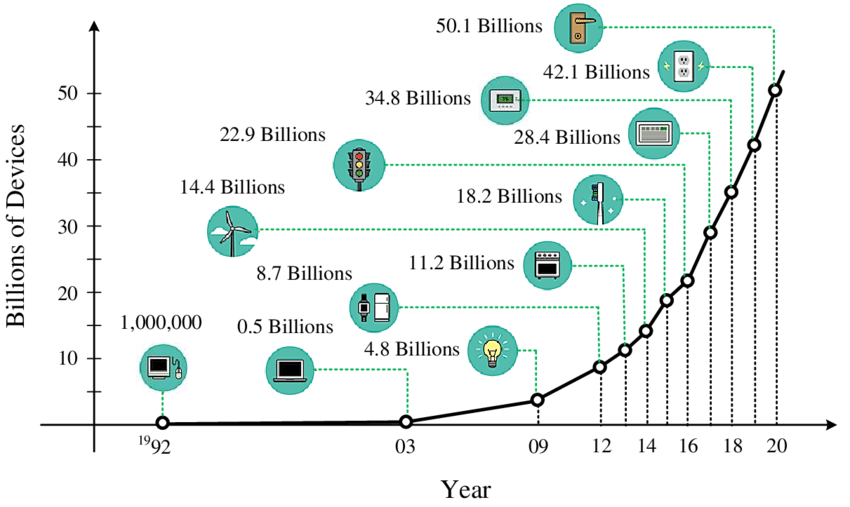
\includegraphics[scale=0.5]{graphics/chapter-1/chap1-number-of-connected-device-to-internet.png}
    \caption{Số lượng thiết bị kết nối vào mạng internet qua các năm \cite{ali2015next}}
    \label{fig:chap1-number-of-connected-device-to-internet}
\end{figure}

\begin{figure}
    \centering
    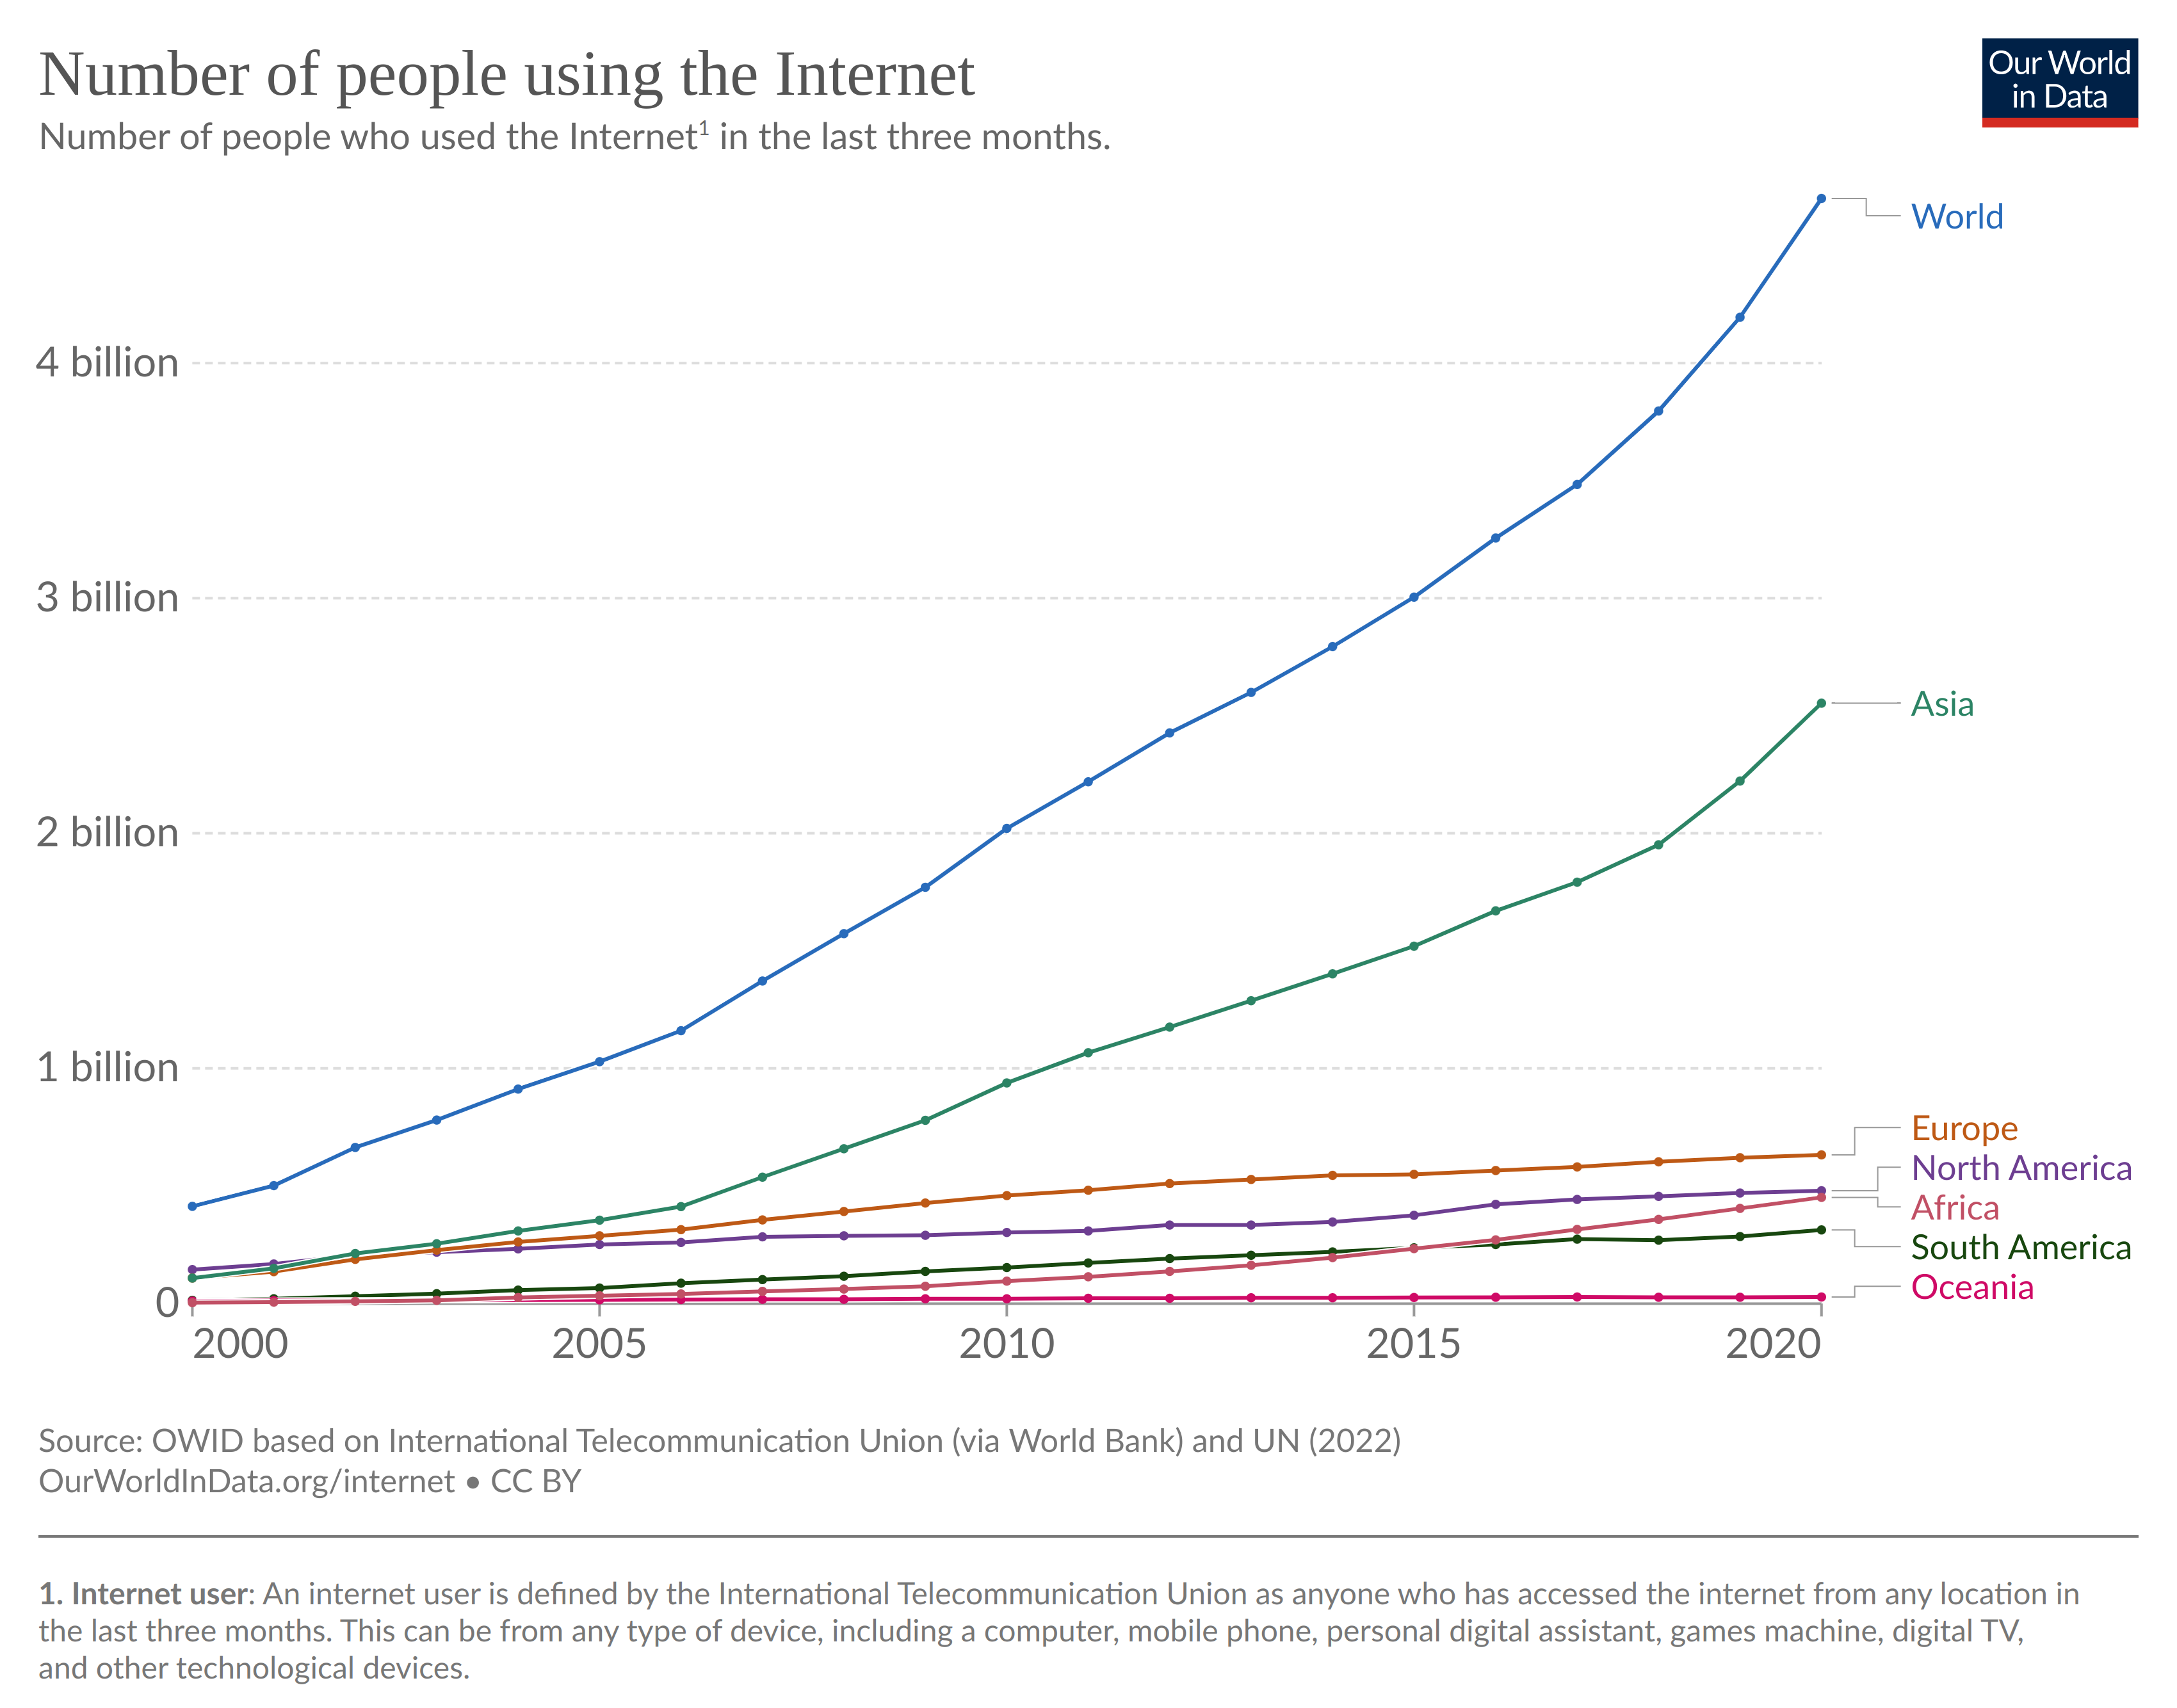
\includegraphics[scale=0.1]{graphics/chapter-1/chap1-number-of-people-use-internet.png}
    \caption{Số lượng người sử dụng internet qua các năm \cite{number2022ourworld}}
    \label{fig:chap1-number-of-people-use-internet}
\end{figure}

Ngoài những yêu cầu cấp thiết về pháp lý, phát triển các biện pháp kỹ thuật là phương thức hiệu quả, áp dụng nhanh chóng và cũng là nguồn quan trọng để có thể  tiếp tục các quy trình pháp luật sau khi bị tấn công. Kiểm thử thâm nhập (penetration testing) là một trong những phương pháp được sử dụng thường xuyên và hiệu quả để đánh giá mức độ an toàn và bảo mật của hệ thống máy tính, giảm thiểu rủi ro liên quan đến bảo mật thông tin \cite{arkin2005software}. 

Kiểm thử xâm nhập nghĩa là, thông qua vai trò như là một hacker, người làm nhiệm vụ thực hiện giả định tấn công vào ứng dụng, máy chủ thực tế, báo cáo kết quả thực hiện và đề xuất những biện pháp bảo vệ dành cho nhà phát triển. Nó có thể được thực hiện trên môi trường thử nghiệm hoặc chính môi trường thực tế. Hiện nay có nhiều công cụ được thiết kế cung cấp khả năng kiểm thử những lỗ hổng cơ bản như Nmap \cite{lyon2009nmap}, Nessus \cite{thacker2006probabilistic}, OpenVAS \cite{aksu2019first}, Metasploit Framework \cite{holik2014effective},... Tuy nhiên để có thể hiểu và phát huy các công cụ này một cách hiệu quả, vẫn cần người sử dụng đã được được đào tạo, có kỹ năng và kiến thức (trong nhiều trường hợp là kinh nghiệm) nhất định. Mặt khác, các hệ thống công nghệ thông tin ngày càng phức tạp, nhiều lớp, nhiệm vụ đánh giá bảo mật theo cách thủ công ngày càng kém hiệu quả, dần dần sẽ không còn khả thi do tỉ lệ sai sót vô ý của con người. 

Như vậy, hiển nhiên cần thiết là quá trình kiểm thử xâm nhập phải được tự động hóa. Không quá dựa nhiều vào công sức của kỹ thuật viên, nhưng cũng không bỏ hoàn toàn họ ra chỉ vì lỗi khách quan (do phải xử lý quá nhiều thông tin và thao tác).

Đây là một chủ đề không mới, nó đã được nghiên cứu nhiều năm nay. Công nghệ phát triển qua từng ngày, kỹ thuật khai thác cũng được thiết kế tinh vi hơn. Từ đó, những lỗ hổng có thể khai thác cũng tăng dần. Vấn đề đặt ra là làm thế nào một công cụ có thể học cách khai thác lỗ hổng và tích lũy kinh nghiệm này cho các lần tiếp theo. Sử dụng máy học là xu hướng hiện nay và kiểm thử  phần mềm cũng không nằm ngoài làn sóng đó. Sử dụng Reinforcement Learning (RL) có thể tận dụng kinh nghiệm thực tế từ các hành động trong quá khứ để quét và tấn công sau đó \cite{liu2020deep}. 




% \begin{figure}[!h]
%     \centering
%     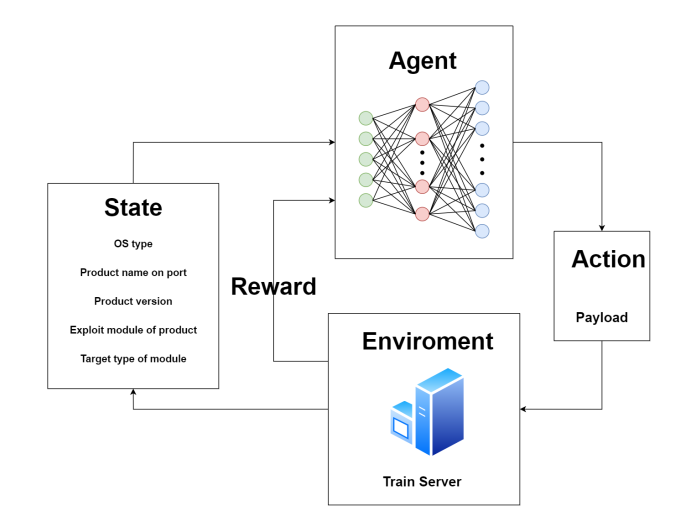
\includegraphics[scale=0.6]{graphics/chapter-1/chap1-abtractRL.png}
%     \caption{Tổng quan về học tăng cường}
%     \label{fig:chap1-abtractRL}
% \end{figure}


% Ví dụ, RL có thể được sử dụng để tạo ra các phần mềm độc hại mới có khả năng làm sai lệch các đánh giá của các công cụ kiểm như như nghiên cứu của nhóm tác giả Daniel Gibert \cite{gibert2022enhancing} hoặc nhóm tác giả Fang \cite{fang2019evading}. Từ đó cho thấy, các hệ thống thông minh dựa trên RL có tính kinh tế, mạnh mẽ, phổ biến và năng động, đặc biệt là về an ninh mạng do sự thay đổi liên tục của các vec-tơ tấn công và payload của chúng \cite{adawadkar2022cyber}. 

% Cho đến nay, đã có một số nghiên cứu liên quan đến các giải pháp tự động hóa kiểm thử thâm nhập bằng cách sử dụng học tăng cường. Trong nghiên cứu của Zhenguo và cộng sự \cite{hu2020automated}, nhóm nghiên cứu đã sử dụng học tăng cường để tìm ra đường tấn công tối ưu nhất cho mô hình mạng thực tế. Các tác giả đã sử dụng công cụ Shodan để thu thập dữ liệu máy chủ thực tế tại các địa điểm công cộng khác nhau để xây dựng các mạng mục tiêu thực tế. Sau đó kết hợp sử dụng MulVAL \cite{yousefi2018reinforcement} và Depth-First Search (DFS) để xây dựng một ma trận tấn công, cuối cùng sử dụng DQN để phân tích ma trận và tìm ra đường tấn công tối ưu nhất cho mô hình mạng. Mặc dù đạt được kết quả tốt theo đánh giá của các tác giả, việc thực hiện vẫn cần rất nhiều sự hỗ trợ từ các framework khác để có thể tự động hóa quá trình thử nghiệm thâm nhập. Trong một nghiên cứu khác, nhóm của Ryusei Maeda \cite{maeda2021automating} cũng đã tập trung vào tấn công tự động với RL sâu, nhưng nghiên cứu này tập trung vào quá trình sau khi bị tấn công. Nghiên cứu này dựa vào một mô-đun agent RL là PowerShell Empire - một mô-đun đã dừng cập nhật - nên nó không thể tiếp tục nghiên cứu và cập nhật sau này.

% Ngoài ra, tại hội nghị Arsenal 2018 Black Hat USA, Isao Takaesu đã giới thiệu DeepExploit \cite{takaesudeepexploit}, một công cụ tấn công tự động sử dụng RL để khai thác các lỗ hổng trên máy chủ. Hiện nay, các thành phần của DeepExploit yêu cầu sửa đổi thêm để hoạt động. Không có thông báo về hiệu suất thực tế của nó đối với các lỗ hổng trong thế giới thực.

% Lấy cảm hứng từ DeepExploit, trong nghiên cứu này, chúng tôi sử dụng thuật toán A3C \cite{mnih2016asynchronous} để huấn luyện agent RL. Nghiên cứu được phát triển nhằm mục đích tích lũy kinh nghiệm trong việc chọn payload chính xác, để khai thác các lỗ hổng có sẵn trong môi trường tiếp theo. Nghiên cứu tập trung vào quá trình do thám và  tấn công trên máy chủ mục tiêu thông qua Metasploit Framework, là hai giai đoạn đầu tiên của quá trình thử nghiệm thâm nhập \cite{engebretson2013basics}. Ngoài ra, sau quá trình thử nghiệm, công cụ sẽ hỗ trợ xuất các báo cáo về các lỗ hổng bị khai thác một cách trực quan, cho phép người dùng dễ dàng quan sát và đánh giá. Cuối cùng, để đánh giá hiệu suất của mô hình, công cụ kiểm tra thâm nhập tự động được áp dụng cho các kiến trúc mạng nơ-ron khác nhau trong các tình huống kế tiếp. 


\section{Mục tiêu của đề tài}

\begin{itemize}
    \item Trong đề tài này, chúng tôi xây dựng một công cụ kiểm thử xâm nhập tự động sử dụng học tăng cường sâu giúp hỗ trợ kỹ thuật viên kiểm thử phần mềm, hỗ trợ xuất báo cáo phục vụ cho nhà phát triển ứng dụng.
    \item 
    Công bố các công trình nghiên cứu khoa học phù hợp với yêu cầu đề tài.
\end{itemize}

\section{Cấu trúc báo cáo}
Nội dung báo cáo của đề tài được tổ chức như sau:
\begin{itemize}
    \item \textbf{Chương \ref{chapter1}} giới thiệu bài toán đặt ra.
    \item \textbf{Chương~\ref{chapter2}} trình bày cơ sở lý thuyết  và các nghiên cứu liên quan.
    \item \textbf{Chương~\ref{chapter3}} trình bày phương pháp và mô hình đề xuất.
    \item \textbf{Chương~\ref{chapter4}} trình bày thực nghiệm và đánh giá.
    \item \textbf{Chương~\ref{chapter5}} tổng kết đề tài và hướng phát triển.
\end{itemize}